\documentclass[titlepage,oneside,11pt]{book}
\author{Nikita Belyavskij}
% Need to add subtitle
\title{EFL Edje Theme Editor 0.5}

\usepackage{xcolor,graphicx}
%\usepackage[bookmarks,pdftex]{hyperref}
%\usepackage[pdftex]{hyperref}
\begin{document}
% generates the title
\maketitle
% insert the table of contents
\tableofcontents
\chapter{Introduction}
%This section should contain general description of EFL them5ing.
\section{Enlightement foundation libraries}
\subsection{Overview}
%short overview of EFL libraries, accordingly to 
%the Edje + Elementary
\subsection{EDC language and Edje library}
%describe flexible way for theming, by using EDC
%language and Edje library mechanism
\subsection{Elementary Theming}
%describe opportunites, that Elementary Theme engine
%give to developers and designers.
\newpage
\section{EFL Edje Theme Editor}
%Eflete is super clever tool. Make user trust to this quote.
\chapter{Installing}
\section{Linux}
\subsection{Dependencies}
\subsection{Upstream git repository}
\subsection{Tarballs}
\subsection{Packages}
\subsubsection{.deb}
\subsubsection{.rpm}
\newpage
\section{MacOS}
\newpage
\section{Windows}
%This section describe installing EFLETE in differrent ways
\chapter{Using the EFL Edje Theme Editor}
\section{Create new project}
EFL Edje theme editor works with projects, that contain resource files, dev file and project file.
Project file describe path to resources and dev file and store metadata abot project. Metadata in project is information about version of product, list of author, license. \newline
Creating new  makes by using wizzard, that help user to fill metadata, chose the project storage directory. Also provide ability to check widgets, which default styles will be included into widget list after creating new project.\newline
For creating new project user can use File menu, or button on toolbar, or use hotkey Ctrl+N.\newline
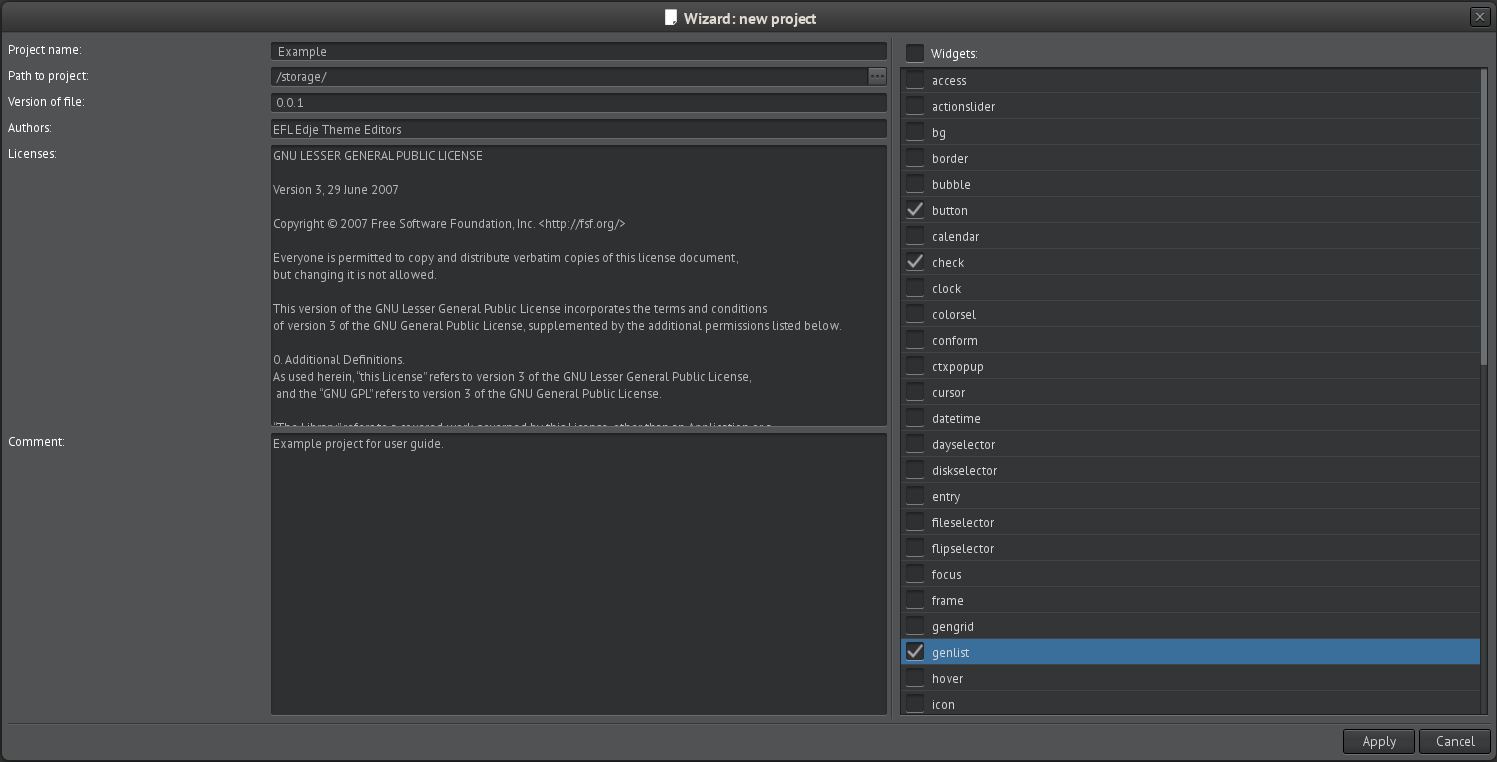
\includegraphics[scale=0.3]{images/wizzard_new_project.png}\newline
In case if needed to create full Elementary theme, checkbox Widgets should be enabled. Be aware, that some of the widgets has dependencies from other. At the creating stage the neccessary widgets will be added automaticaly.

After successfull create new project, view will be switched to the edit mode. HERE should be link to the section Edit project %\refchapter
\section{Import project}
EFL Edje Theme Editor support creating new project from already existed data files.
User can import project from edc files or from edj binary.
\subsection{EDC project}
Importing from project from edc files requre knows pathes for all resources, that used in project. It mean that some of pathes to the resources (such as images, sounds, data files, etc) lost - project creation will failed.
Import data drom edc files is possible by using wizzard "{}import edc"{}.\newline
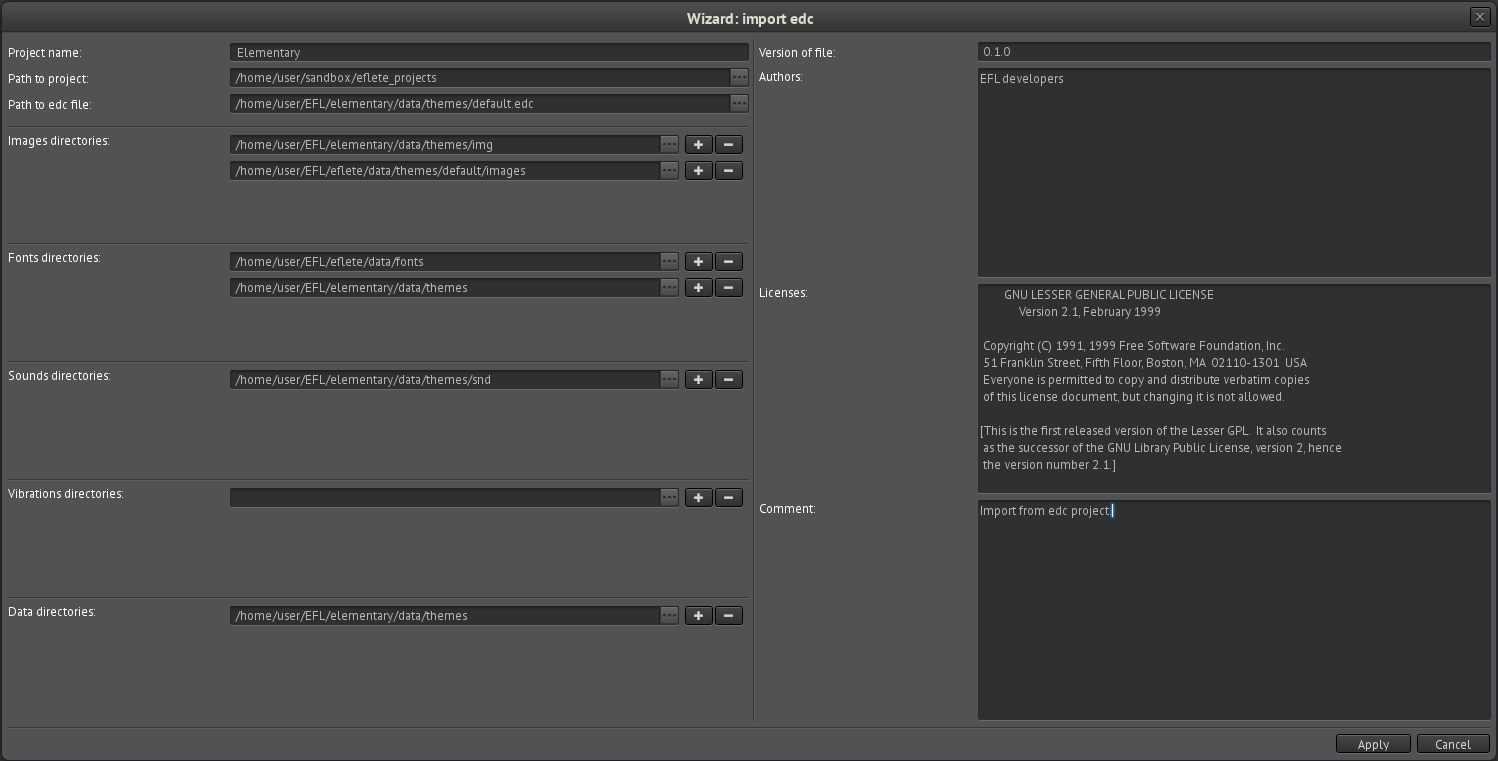
\includegraphics[scale=0.3]{images/wizzard_import_edc.png}\newline 
Process of edit newly imported project is the same as in New project way.
\subsection{EDJ project}
In case when present binary theme file (that have extension *.edj) should be used EDJ project importing. This action initiate decompiling resources from the binary file into project directories. Accordingly to this process, resource files, that marked as external, should present in directories.
Using "{}import edj"{} wizzard requare edj file placement and directory path, where new project will store. Editing project is the same as in other ways.
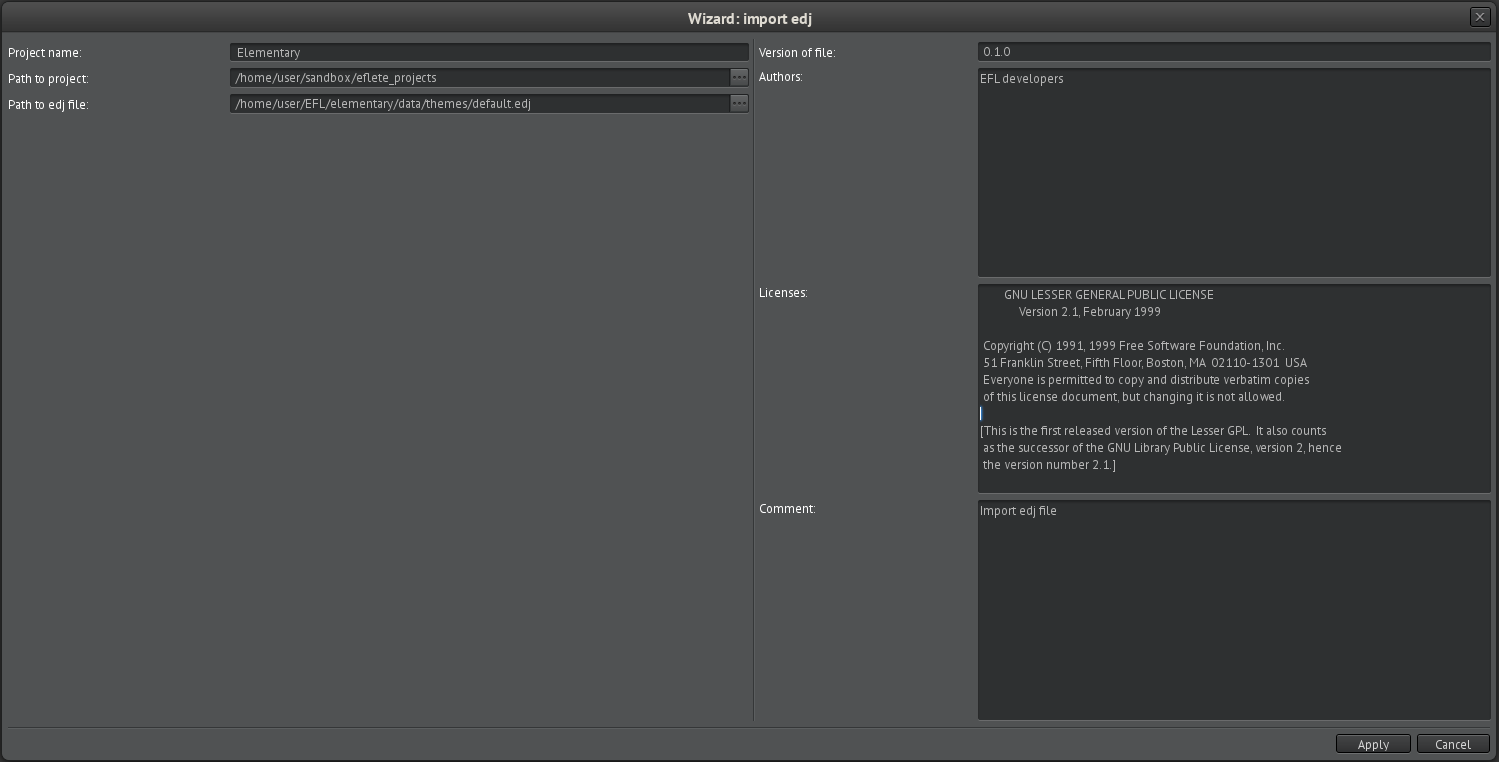
\includegraphics[scale=0.3]{images/wizzard_import_edj.png}\newline 
\section{Resource management}
EFL Edje Theme Editor tool provide build-in mangeres for different kind of resource.
\subsection{Images}
One of the most important type of resource, that uses in EFL themes and layouts is images. \newline
For add/delete images in project Eflete provide "{}Image manager"{}.\newline
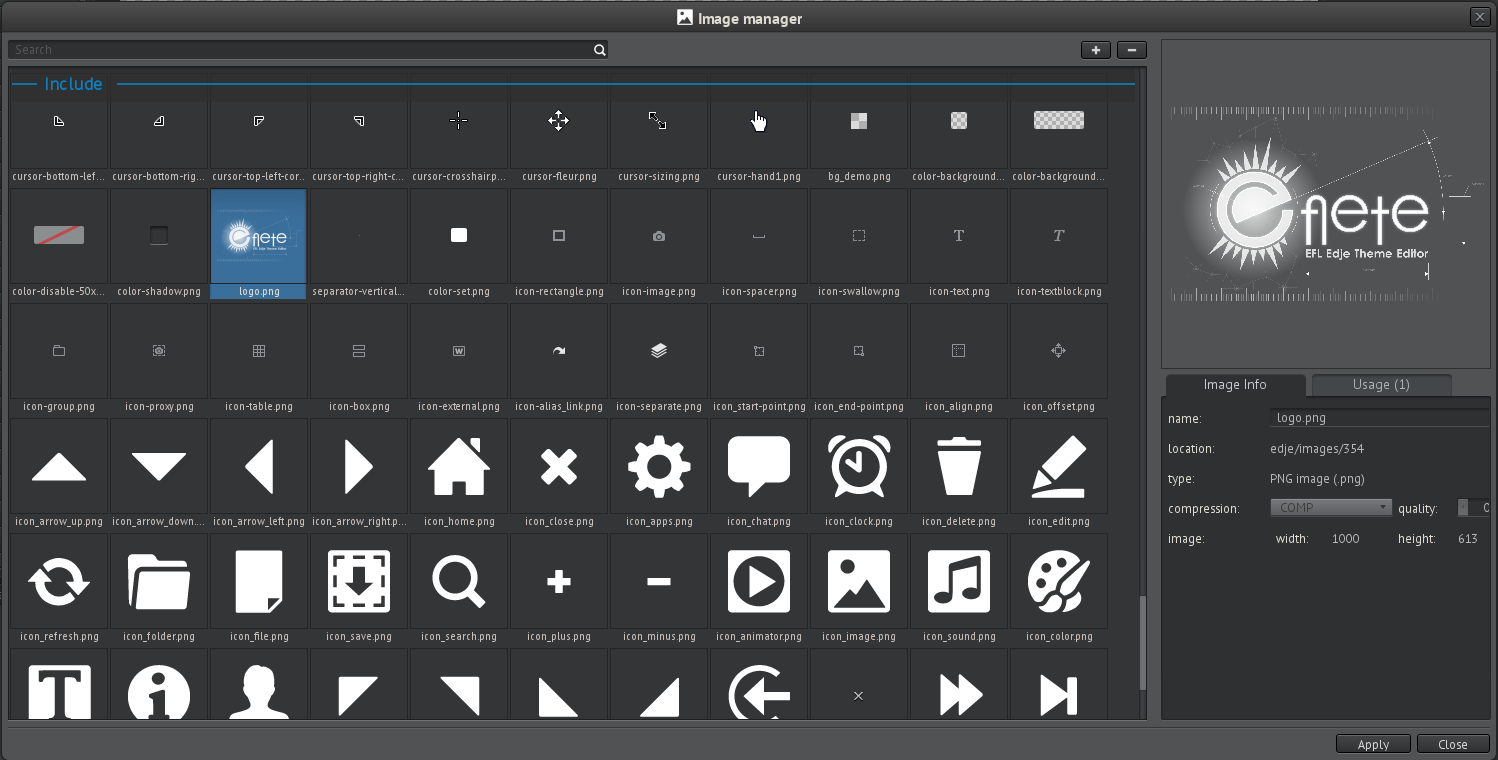
\includegraphics[scale=0.3]{images/image_manager_main.png}\newline
In this present all image resources, that uses in project. All images sorted by alphabet. "{}Find"{} bar make search neccesary image fast. Short file information at the right side of manager contain preview (note: preview does not appear any kind of anti alising or smoothing).\newline
%place here some images with preview examples. How this images llok in 3rd party viewers in compare with image manager preview
\newline Below preview block placed information about image file, such as file name, width, heigth, type and etc. Image usage information is placed inside second tab.\newline
%add examples where this is can be usefull
\newline
Image manager also uses for choosing images in part attributes (such as normal image, or tweens).
More information about image manager features written at 4.3.1.
\subsection{Sounds}
Edje library provide playing media files. Eflete also support sound resources. It can be ogg, wav or flac files. Concept of usage sound manger is the same as image manger. Here present ability to add new resource files or tones. All sound resources separeted into two groups: sounds and tones. At the right side of the "{}sound manager"{} placed player, that can play any selected resource item. Below media block placed information about selected item. Here the same rules as in "{}image manager"{}.\newline
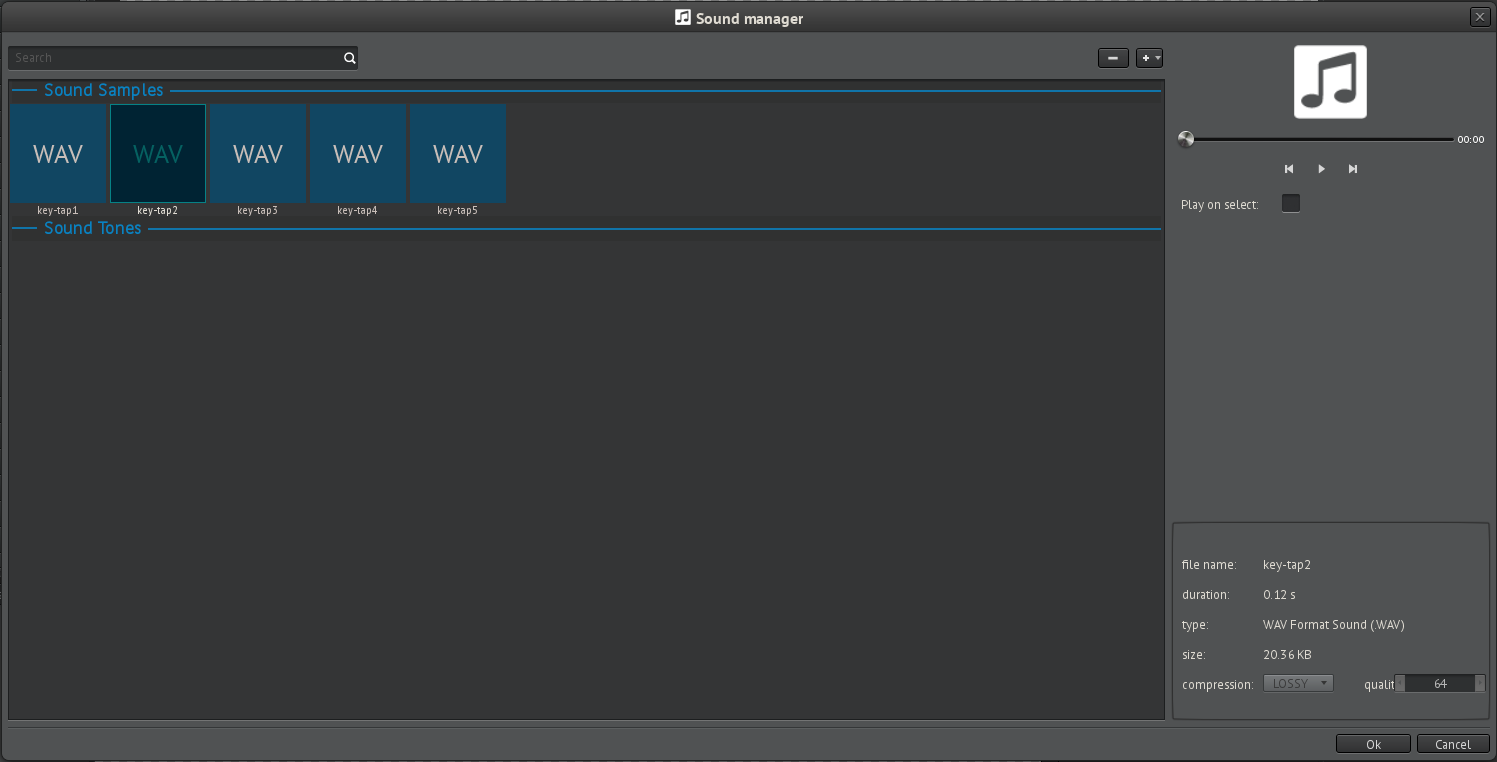
\includegraphics[scale=0.3]{images/sound_manager_main.png}\newline
%replace with screenshot, that contain sound manger with a lot of different types of samples and tones.
Additional information about "{}sound manager"{} UX placed at section 4.3.2
\subsection{Color classes}
Some themes are color depends, it mean that set of styles and layouts use one or more main colors. In case, when main colors are changed happens issue: change color of each part in each style. And what if theme contain hundred of styles and thousens parts? Edje library provide color classes feature. Once defined color class, that used in parts can be changed. And all parts will change it colors automaticaly. EFL Edje Theme editor provide internal tool, that named "{}color class manger"{}. It is very simple and useful manager/\newline
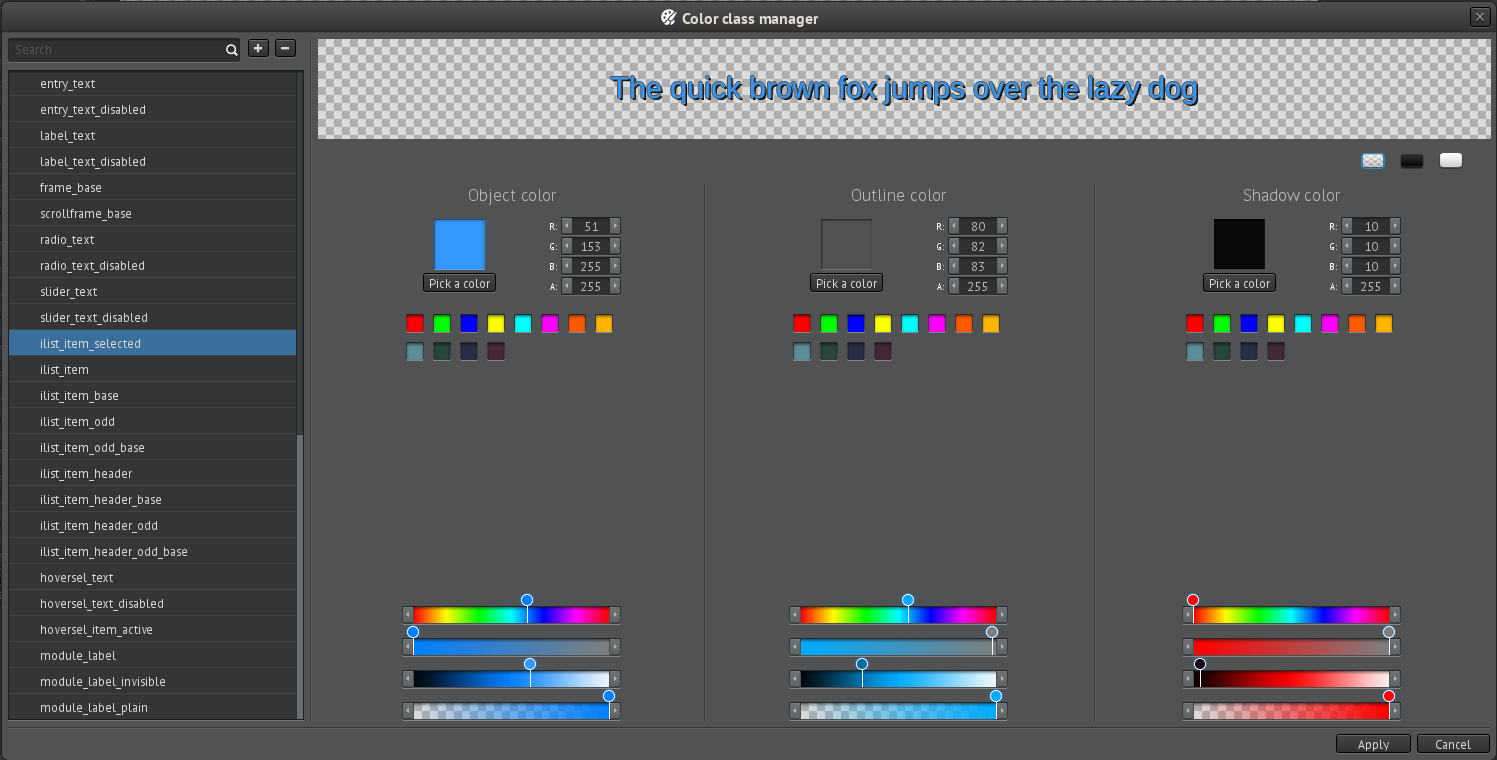
\includegraphics[scale=0.3]{images/colorclass_manager_main.png}\newline
Created color classe in "{}color class manager"{} are avalaible in part attributes.
More information about "{}colorclass manager"{} features written at 4.3.3.
\subsection{Textblock styles}
Edje library provide ability to use HTML-like tags inside textblock primitives. Usauly notifications requare to make accent on important word inside message. Or highlight some text, like in code editors. Use text styles make it possibe.\newline
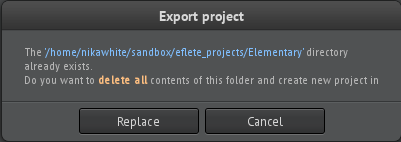
\includegraphics[scale=0.5]{images/textblock_style_example_1.png}\newline 
Notification about deleting directory.\newline
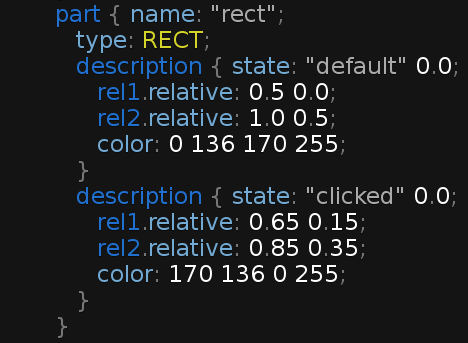
\includegraphics[scale=0.5]{images/textblock_style_example_2.png}\newline
Using textblock styles in the Enventor application.\newline
The "{}textblock style manager"{} provide user interface for easy management styles, tags and attributes. Creating new and edit already exists styles without writting a lot of paramters of text format is main task of this manager.\newline
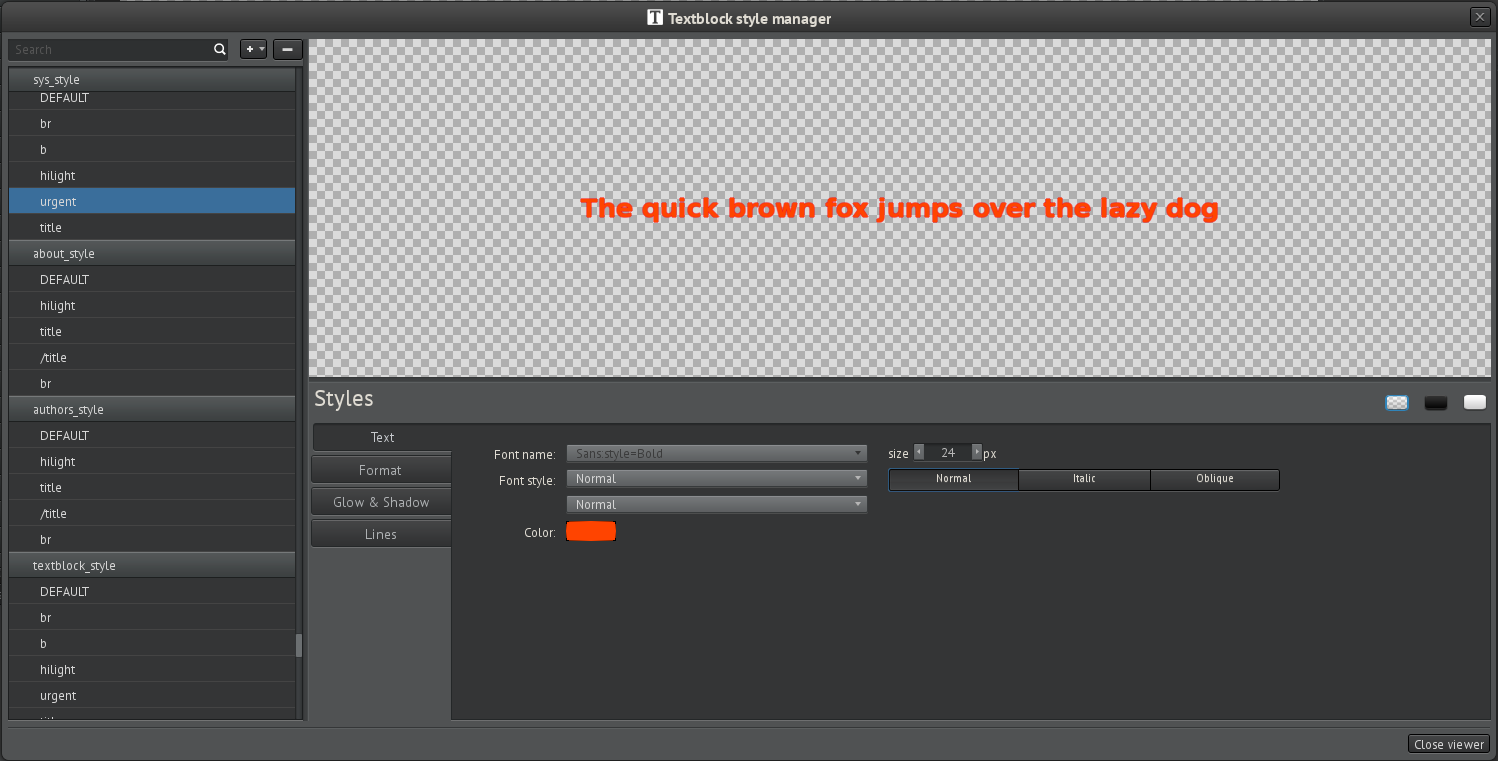
\includegraphics[scale=0.3]{images/textblock_manager_main.png}\newline
More information about "{}textblock style manager"{} features written at 4.3.4.
\section{Edit project}
\subsection{Styles}
\subsection{Layouts}
\subsection{Parts}
\subsubsection{States}
\subsubsection{Attributes}
\subsection{Programs}
\subsection{Workspace}
\section{Live preview}
\section{History}
\section{Enventor mode}
\section{Export}
\subsection{Export as EDJ}
\subsection{Export as EDC}
\chapter{User interface}
\section{Main screen}
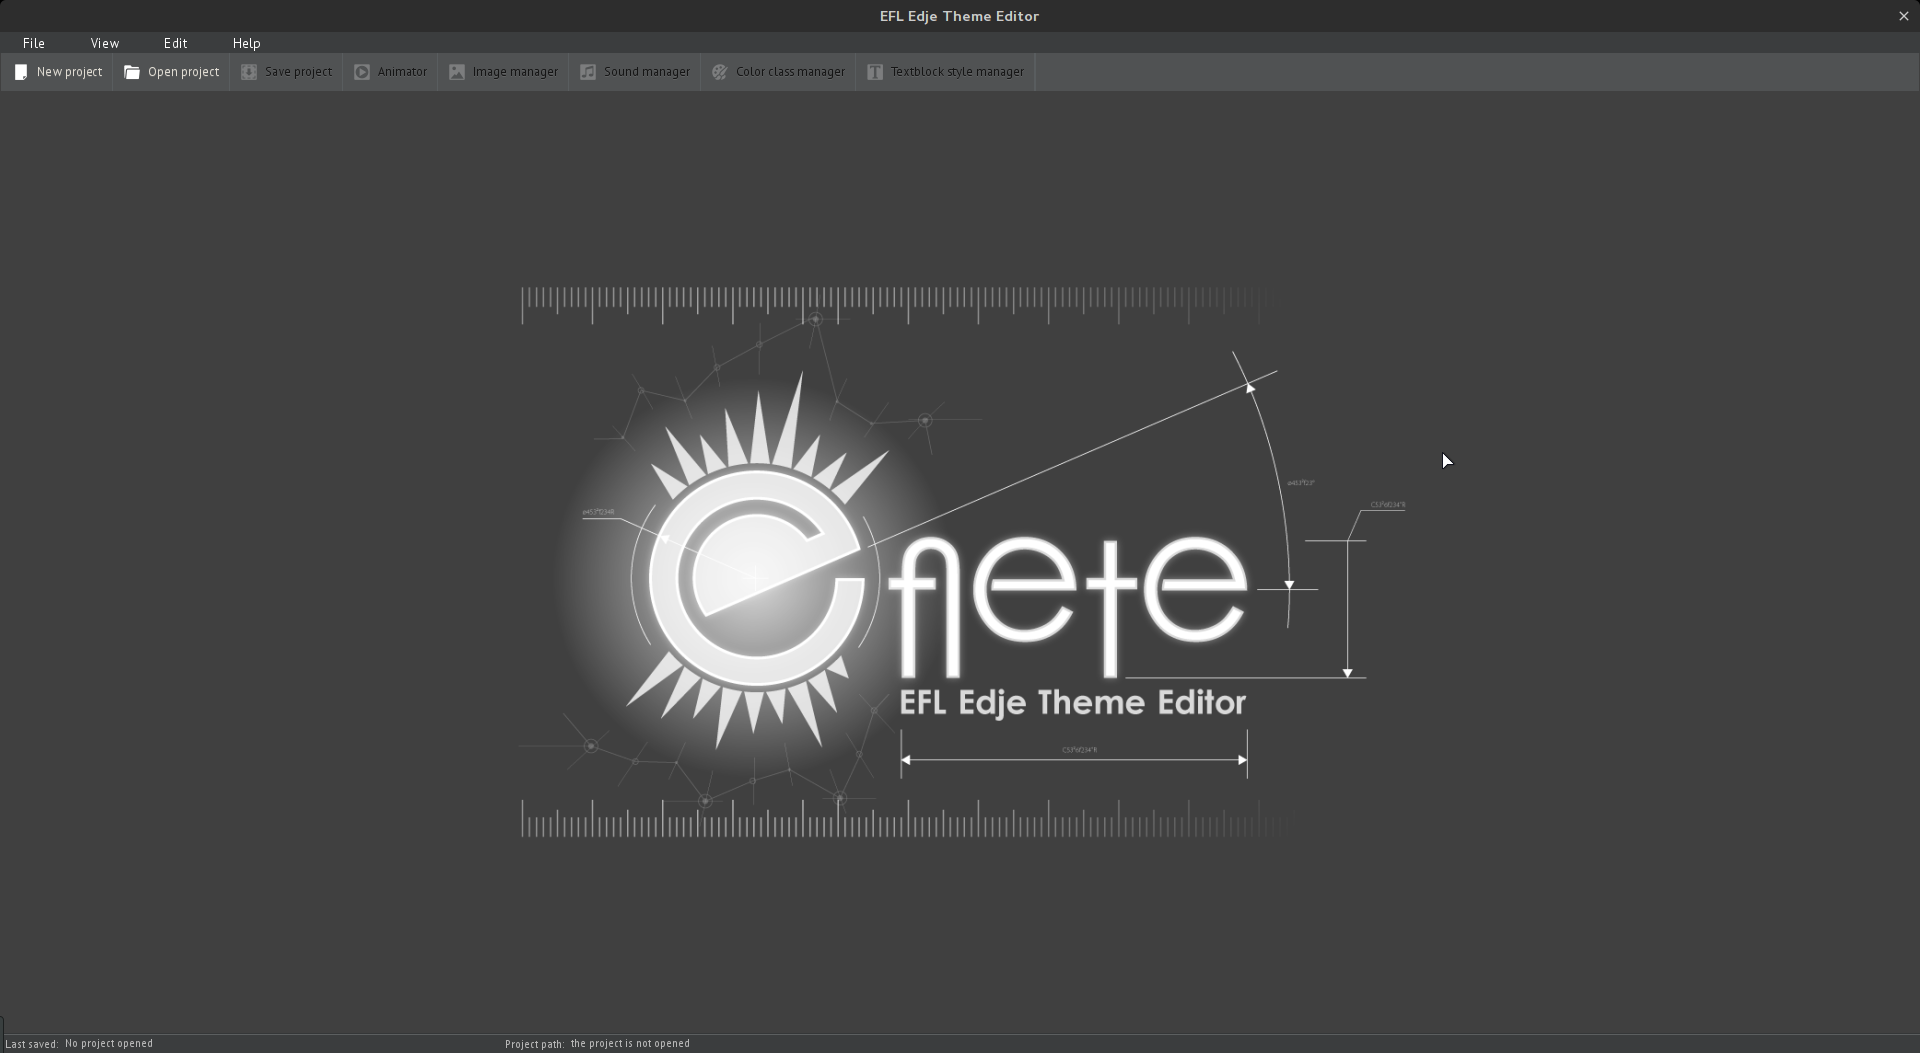
\includegraphics[scale=0.2]{images/main_screen.png}
Main screen contain component, that always accesseble to user. Here is: main menu, tollbar with fast access buttons, status bar.
\subsection{Main menu}

\includegraphics{images/main_menu.png}
\subsubsection{File}
File menu provide ability to manage project. 
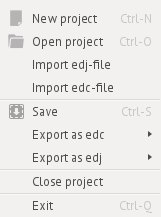
\includegraphics{images/file_menu.png}
Export as edc submenu

\includegraphics{images/file_export_as_edc_submenu.png}
User can export whole project to edc files tree or export only currently opened group into one single edc file and resource directories.
\subsubsection{View}
View section is provide ability to manipulate apperance of workspace area.
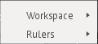
\includegraphics{images/view_menu.png}
Functionality of changing zoom fsctor or switching beetwen views on the workspace is placed in workspace submenu.
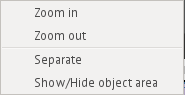
\includegraphics{images/view_workspace_submenu.png}
Manipulating rulers functions placed in rulers submenu
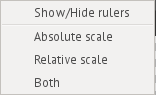
\includegraphics{images/view_rulers_submenu.png}
\subsection{Toolbar}
%describe toolbar buttons
\subsection{Statusbar}
\subsection{Lists}
\subsubsection{Widgets}
\subsubsection{Layouts}
\subsubsection{Parts}
\subsubsection{Items}
\subsubsection{State}
\subsubsection{Signal}
\subsection{Attributes}
\subsubsection{Layout}
\subsubsection{Part}
\subsubsection{State}
\subsubsection{Object area}
\subsubsection{Fill}
\subsubsection{Image}
\subsubsection{Table}
\subsubsection{Box}
\subsubsection{Text}
\subsubsection{Textblock}
\subsection{Enventor mode}
\section{Wizzards}
\subsection{New project}
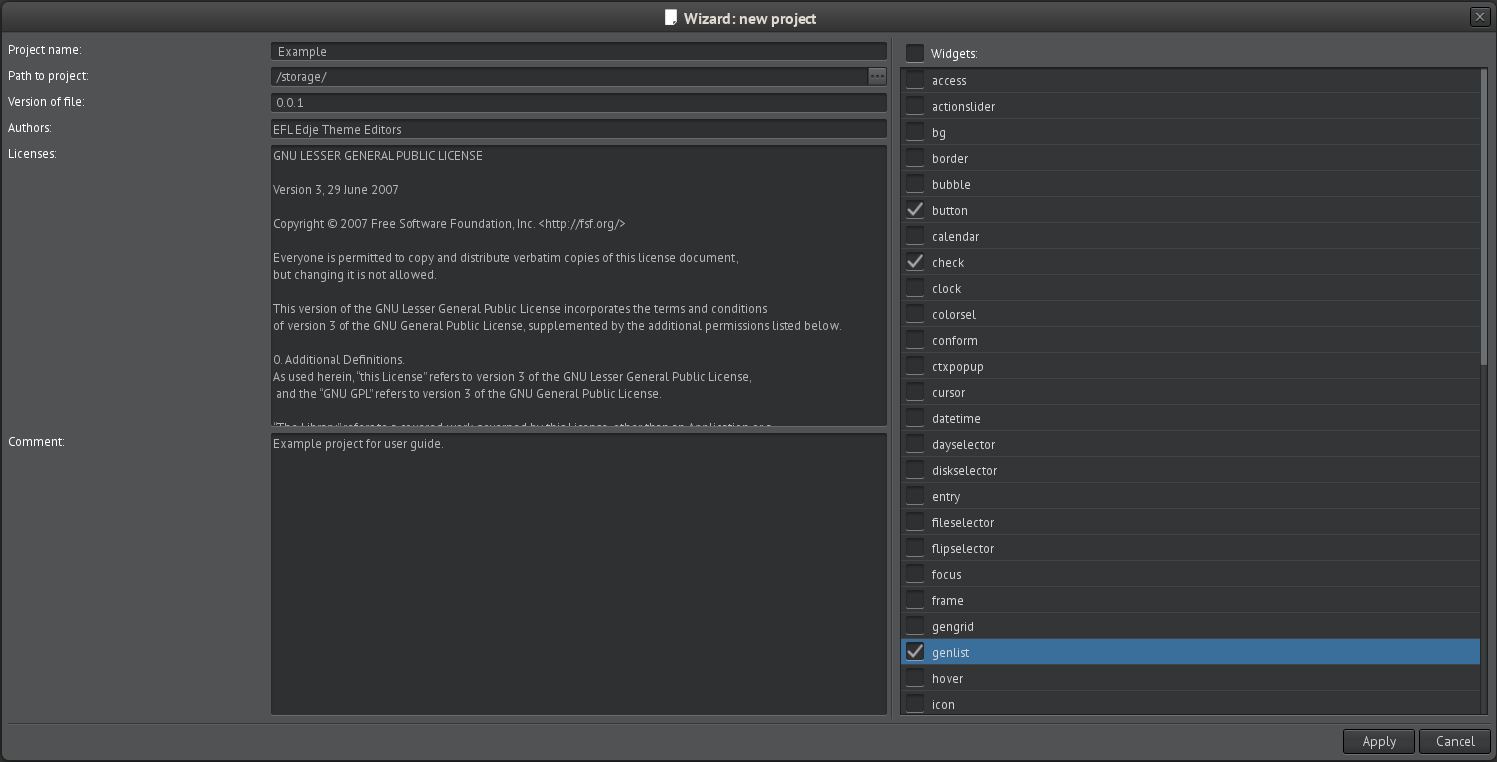
\includegraphics[scale=0.2]{images/wizzard_new_project.png}\newline
\subsection{Import edc}
\subsection{Import edj}
\section{Resource managers}
\subsection{Images}
\subsection{Sounds}
\subsection{Color classes}
\subsection{Textblock styles}
\section{Animator}
\subsection{Program editor}
\subsection{Animator}
\section{Workspace}
\subsection{View modes}
\subsection{Rulers}
\subsection{Context menu}
\subsubsection{Zoom}
\subsubsection{Rulers}
\subsection{Edit mode}
\subsubsection{Resize}
\subsubsection{Aligment}
\section{History}
\chapter{Appendix}
\section{Hotkeys}
\section{Example application}
%Describe little thing like hotkeys, tips and examples
\end{document}